\section{Finite element analysis}
\label{sec:metapde-fea}
PDEs are most naturally posed in a \emph{strong form}:
\begin{align}
\mathcal{F}(u)(x) &= 0 \quad &\text{in } \Omega, \label{eq:metapde-strongform} \\
\mathcal{G}(u)(x) &= 0 \quad &\text{on } \partial \Omega. \label{eq:metapde-bc}
\end{align}
where $\Omega \subset \mathbb{R}^{d_\Omega}$ is the problem domain with boundary $\partial \Omega$, $u: \Omega \to \mathbb{R}^{d_u}$
is the solution,
$\mathcal{F}: (\Omega \to \mathbb{R}^{d_u}) \to (\Omega \to \mathbb{R}^{d_\mathcal{F}})$
is a linear or nonlinear operator involving $u$ and its
partial derivatives, and
$\mathcal{G}: (\Omega \to \mathbb{R}^{u}) \to (\Omega \to \mathbb{R}^{d_\mathcal{G}})$
is an operator enforcing a boundary condition
(for example, $\mathcal{G}(u)(x) = u(x) - b(x)$ is a Dirichlet boundary condition
forcing $u$ to be equal to a function $b$ on the boundary).

Finite element analysis involves rewriting the PDE in a \emph{weak form}:
find $u$ in a function space $\mathcal{V}$, such that
\begin{align}
\int_{\Omega} <\mathcal{F}(u)(x), v(x)> dx + \int_{\partial \Omega} <\mathcal{G}(u)(x), v(x)> dx &= 0 \quad \forall v \in \mathcal{V} \label{eq:metapde-eakform}
\end{align}
When $\mathcal{V}$ is a suitable infinite-dimensional Sobolev space,
we recover the same solution as the strong form.
In order to solve the problem numerically with FEA,
we let $\mathcal{V}$ be a class of piecewise low-degree polynomials over the domain,
parameterized by some finite number of interpolating points.
We fix the values of the interpolating points on the boundary, form a set of basis
vectors $v$ for $\mathcal{V}$, rewrite the weak form of the PDE as a linear or
nonlinear system representing the set of constraints that must be satisfied,
and solve the system with an appropriate linear or nonlinear solver.
Figure \ref{fig:metapde-poisson} shows as an example the Poisson problem on a disc.
For this simple problem we have $\mathcal{F}(u) = \nabla \dot{} \nabla u - f$, for
a spatially varying source term $f$, and $\mathcal{G}(u) = u$, i.e. enforcing $u=0$
on the boundary.

\begin{figure}[t]
  \centering
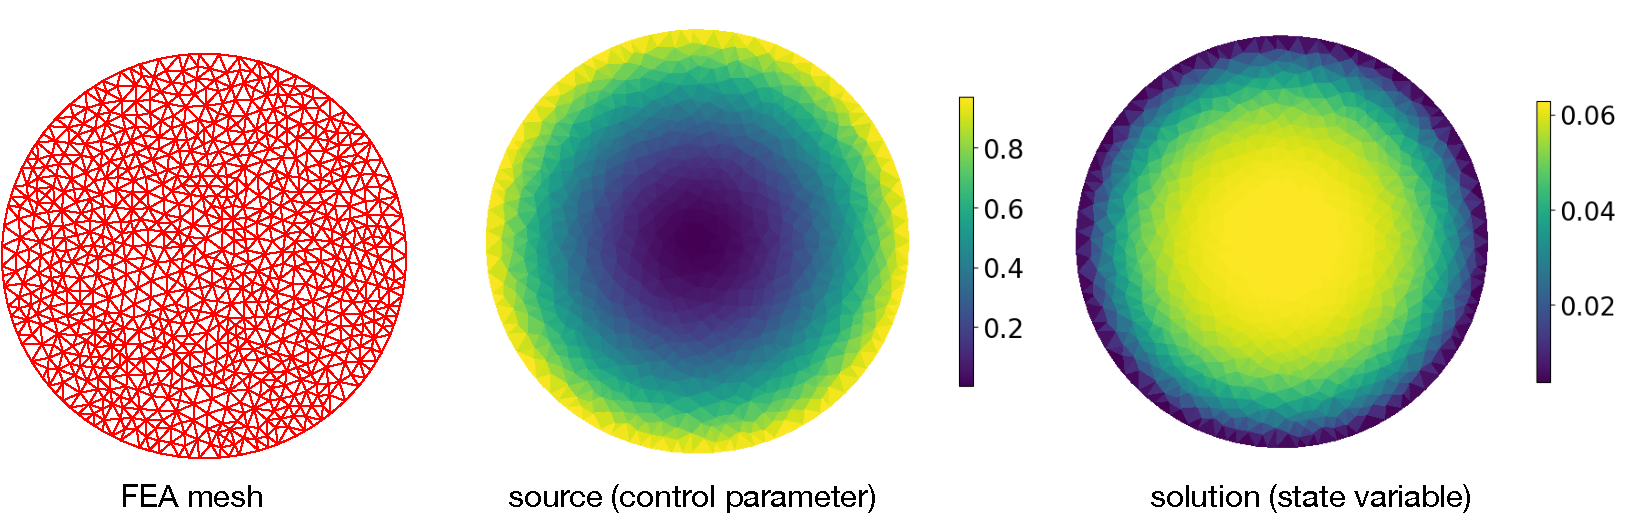
\includegraphics[width=10cm]{figures/poisson_equation.pdf}
\caption{\small Poisson equation on a disc.
Figure: \citet{xue2020amortized}.}%
\label{fig:metapde-poisson}%
\end{figure}

We observe that finding the solution to the PDE i equivalent to finding
the minimizer of the variational energy
\begin{align*}
  \mathcal{J}(u) &= \int_{\Omega} ||\mathcal{F}(u)(x)||^2_2 dx +
  \int_{\partial\Omega} ||\mathcal{G}(u)(x)||_2^2 dx
\end{align*}
As with \citet{xue2020amortized}, we use this optimization perspective
to derive an efficient training method for our surrogate models.
